\subsection{Introduction}
According to \cite{yoshiyuki1995nms} the renormalization algorithm works best
when the cities are uniformly distributed over the pane. It is clear that this
is very unlikely in real TSP optimisation problems. For the United States of
America for example most cities are located on the east coast. The Netherlands
on the other hand have a concentration of cities in the west of the country.
It is clear that the location of the cities cannot be changed without
modifying the problem. We propose to change the distribution of the cities
over the cells in the grid by rotating the grid used by the renormalization
process.

A deterministic algorithm such as a greedy algorithm, can be used to find the
angle of the rotation leading to the best approximation of the shortest route. Yet
deterministic algorithms will succumb to stay in a local optimum and are
therefore inadequate. Probabilistic algorithms can resist to this risk. By
first seeking through the entire sample space multiple optima can be found.
Depending on the algorithm used one or more optima are further analyzed to
find a global optimum.

The thermodynamic simulated annealing algorithm \cite{devicente2003pts}~is the
probabilistic algorithm used in this work. This process is an extension of the
simulated annealing algorithm first discussed in \cite{kirkpatrick83}. The
latter algorithm is analogous to the process of annealing in metallurgy. First
a metal is heated to high temperature. Once warm it is slowly cooled in a
controlled way permitting the atoms of the metal to fall into an optimal
equilibrium and thereby reducing the energy to a minimum. Because the atoms
are in an optimal place the metal has many ideal properties. 

To use simulated annealing first some properties of the system have to be
defined to resemble the physical process. The energy of the system is defined
to be the length of the route found by the renormalization process. The sample
space which can be altered to reduce the energy is the angle of the rotation of the grid.
The two core elements of the simulated annealing process are the cooling
schedule which permits to reduce the energy of the system. The second is the
method used to bring the system in a new disequilibrium. This latter property,
to which will be referred to as the perturbation function, models the dynamic of
the atoms depending of the temperature of the system.

The next subsections treat the perturbation function and the cooling schedule used
to find the optimal angle of the rotation.

\subsection{Perturbation function}
In most simulated annealing algorithms the system is brought in a new
disequilibrium by changing the current state by a small fraction. This is hard
to accomplish when rotating the grid used by the renormalization algorithm;
even a very small change of the angle of the rotation can lead to a complete
new route with a much higher or lower energy. Yet if the perturbation function
allows to return in the previously better state this is not a problem. To
implement this behaviour the perturbation function uses a random walk.

\newcommand{\expt}{\ensuremath{\mathbb{E}}}
The random walk used is based on a Brownian motion\cite{brown1829bam}. The
Brownian motion is used, among others, in physics to describe the random
movement of particles suspended in a fluid. The Brownian motion is
a stochastic process $\lbrace W_t\rbrace_{t\geq 0}$ with the properties that
if $\mathcal{F}_t$ denotes the information known until time $t$ then 
$\expt(W_{t + 1}\mid \mathcal{F}_t) = \expt(W_t \mid \mathcal{F}_t)$ i.e. the
expectation of process at the next time step is only dependent on the
information known up to the current time. However the expectation is still
zero. Furthermore, $W_t - W_s \sim N(0, 1)$. Using this process we define the
angle of rotation $\theta_t$ at time $t$ to be:
\begin{equation}\label{eq:rot}
\theta_{t + 1} = \theta_{t} + \alpha 2\pi\frac{T - T_{end}}
	{T_{init} - T_{end}}W_t
\end{equation}
where $T_{init}, T_{end}$ and $T$ are respectively the initial temperature of
the system, the desired end temperature and the current temperature. The
factor $\alpha$ is used to determine how much the rotation should be influenced
by the Brownian motion. The Brownian motion is multiplied by $2\pi$ to ensure
that an entire rotation can be accomplished.

\ctable[caption={The rotation at various times},
	     figure,
		  label={fig:rotful}]{c}{\tnote[]{}}{\FL
		  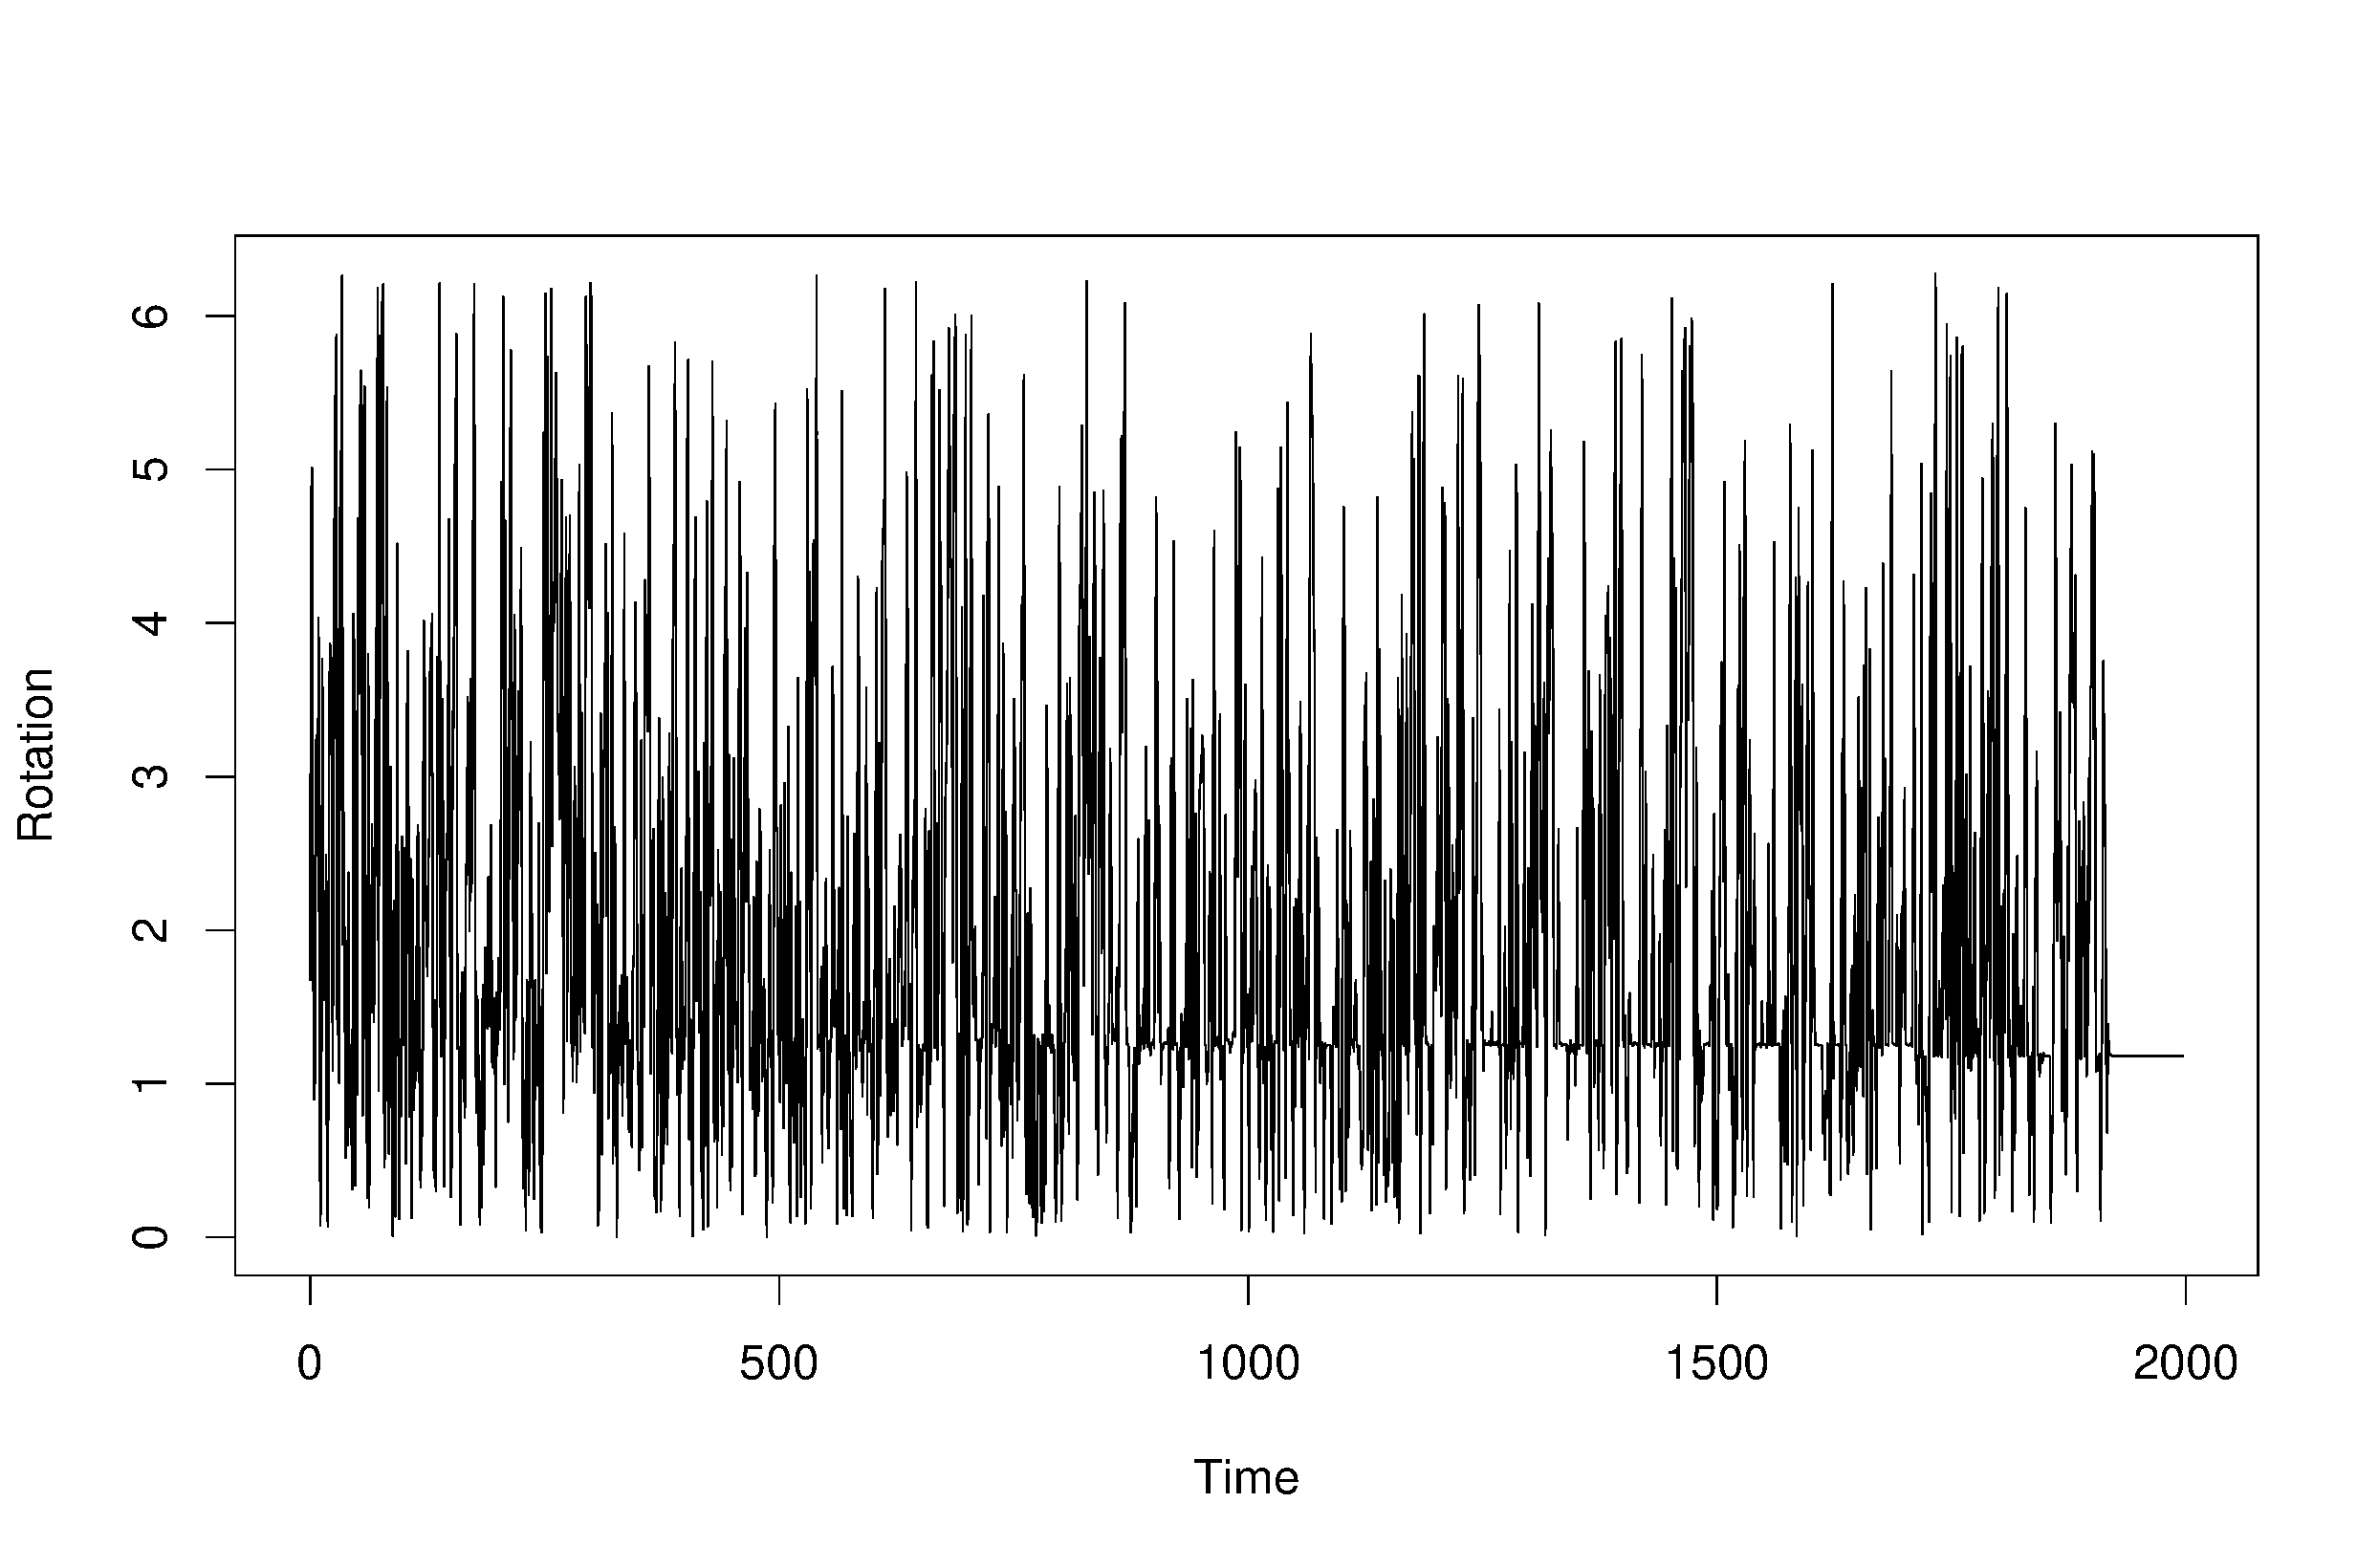
\includegraphics[width=7cm]{fig/rotation_full}\NN
		  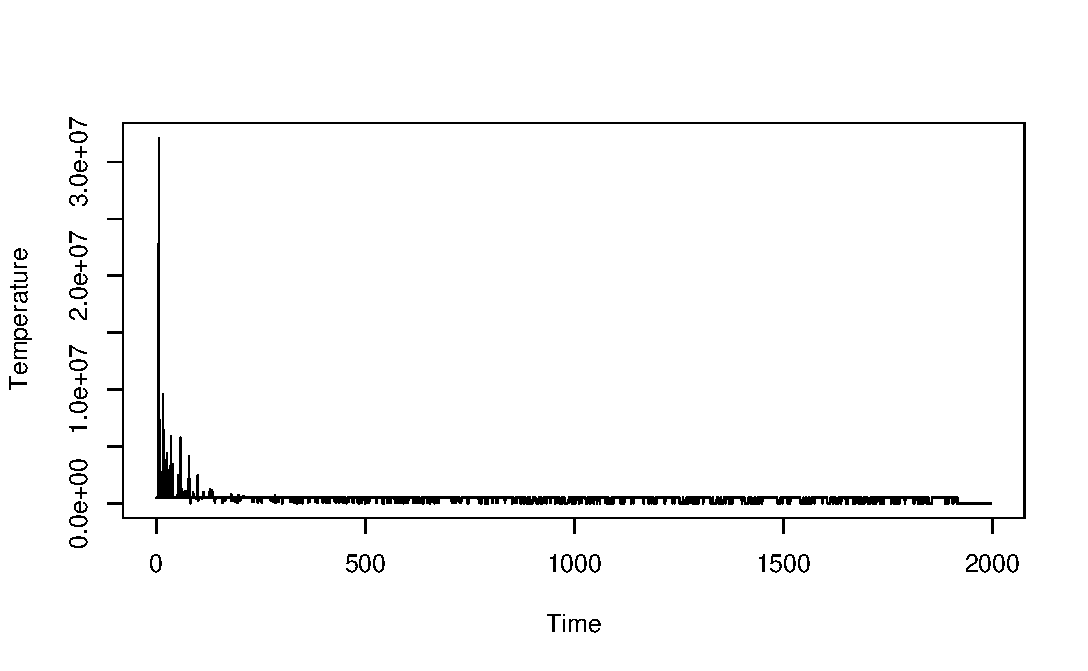
\includegraphics[width=7cm]{fig/temp_rot_full}\LL
		  }

\ctable[caption={The rotation at various times},
	     figure,
		  label={fig:rot46}]{c}{\tnote[]{}}{\FL
		  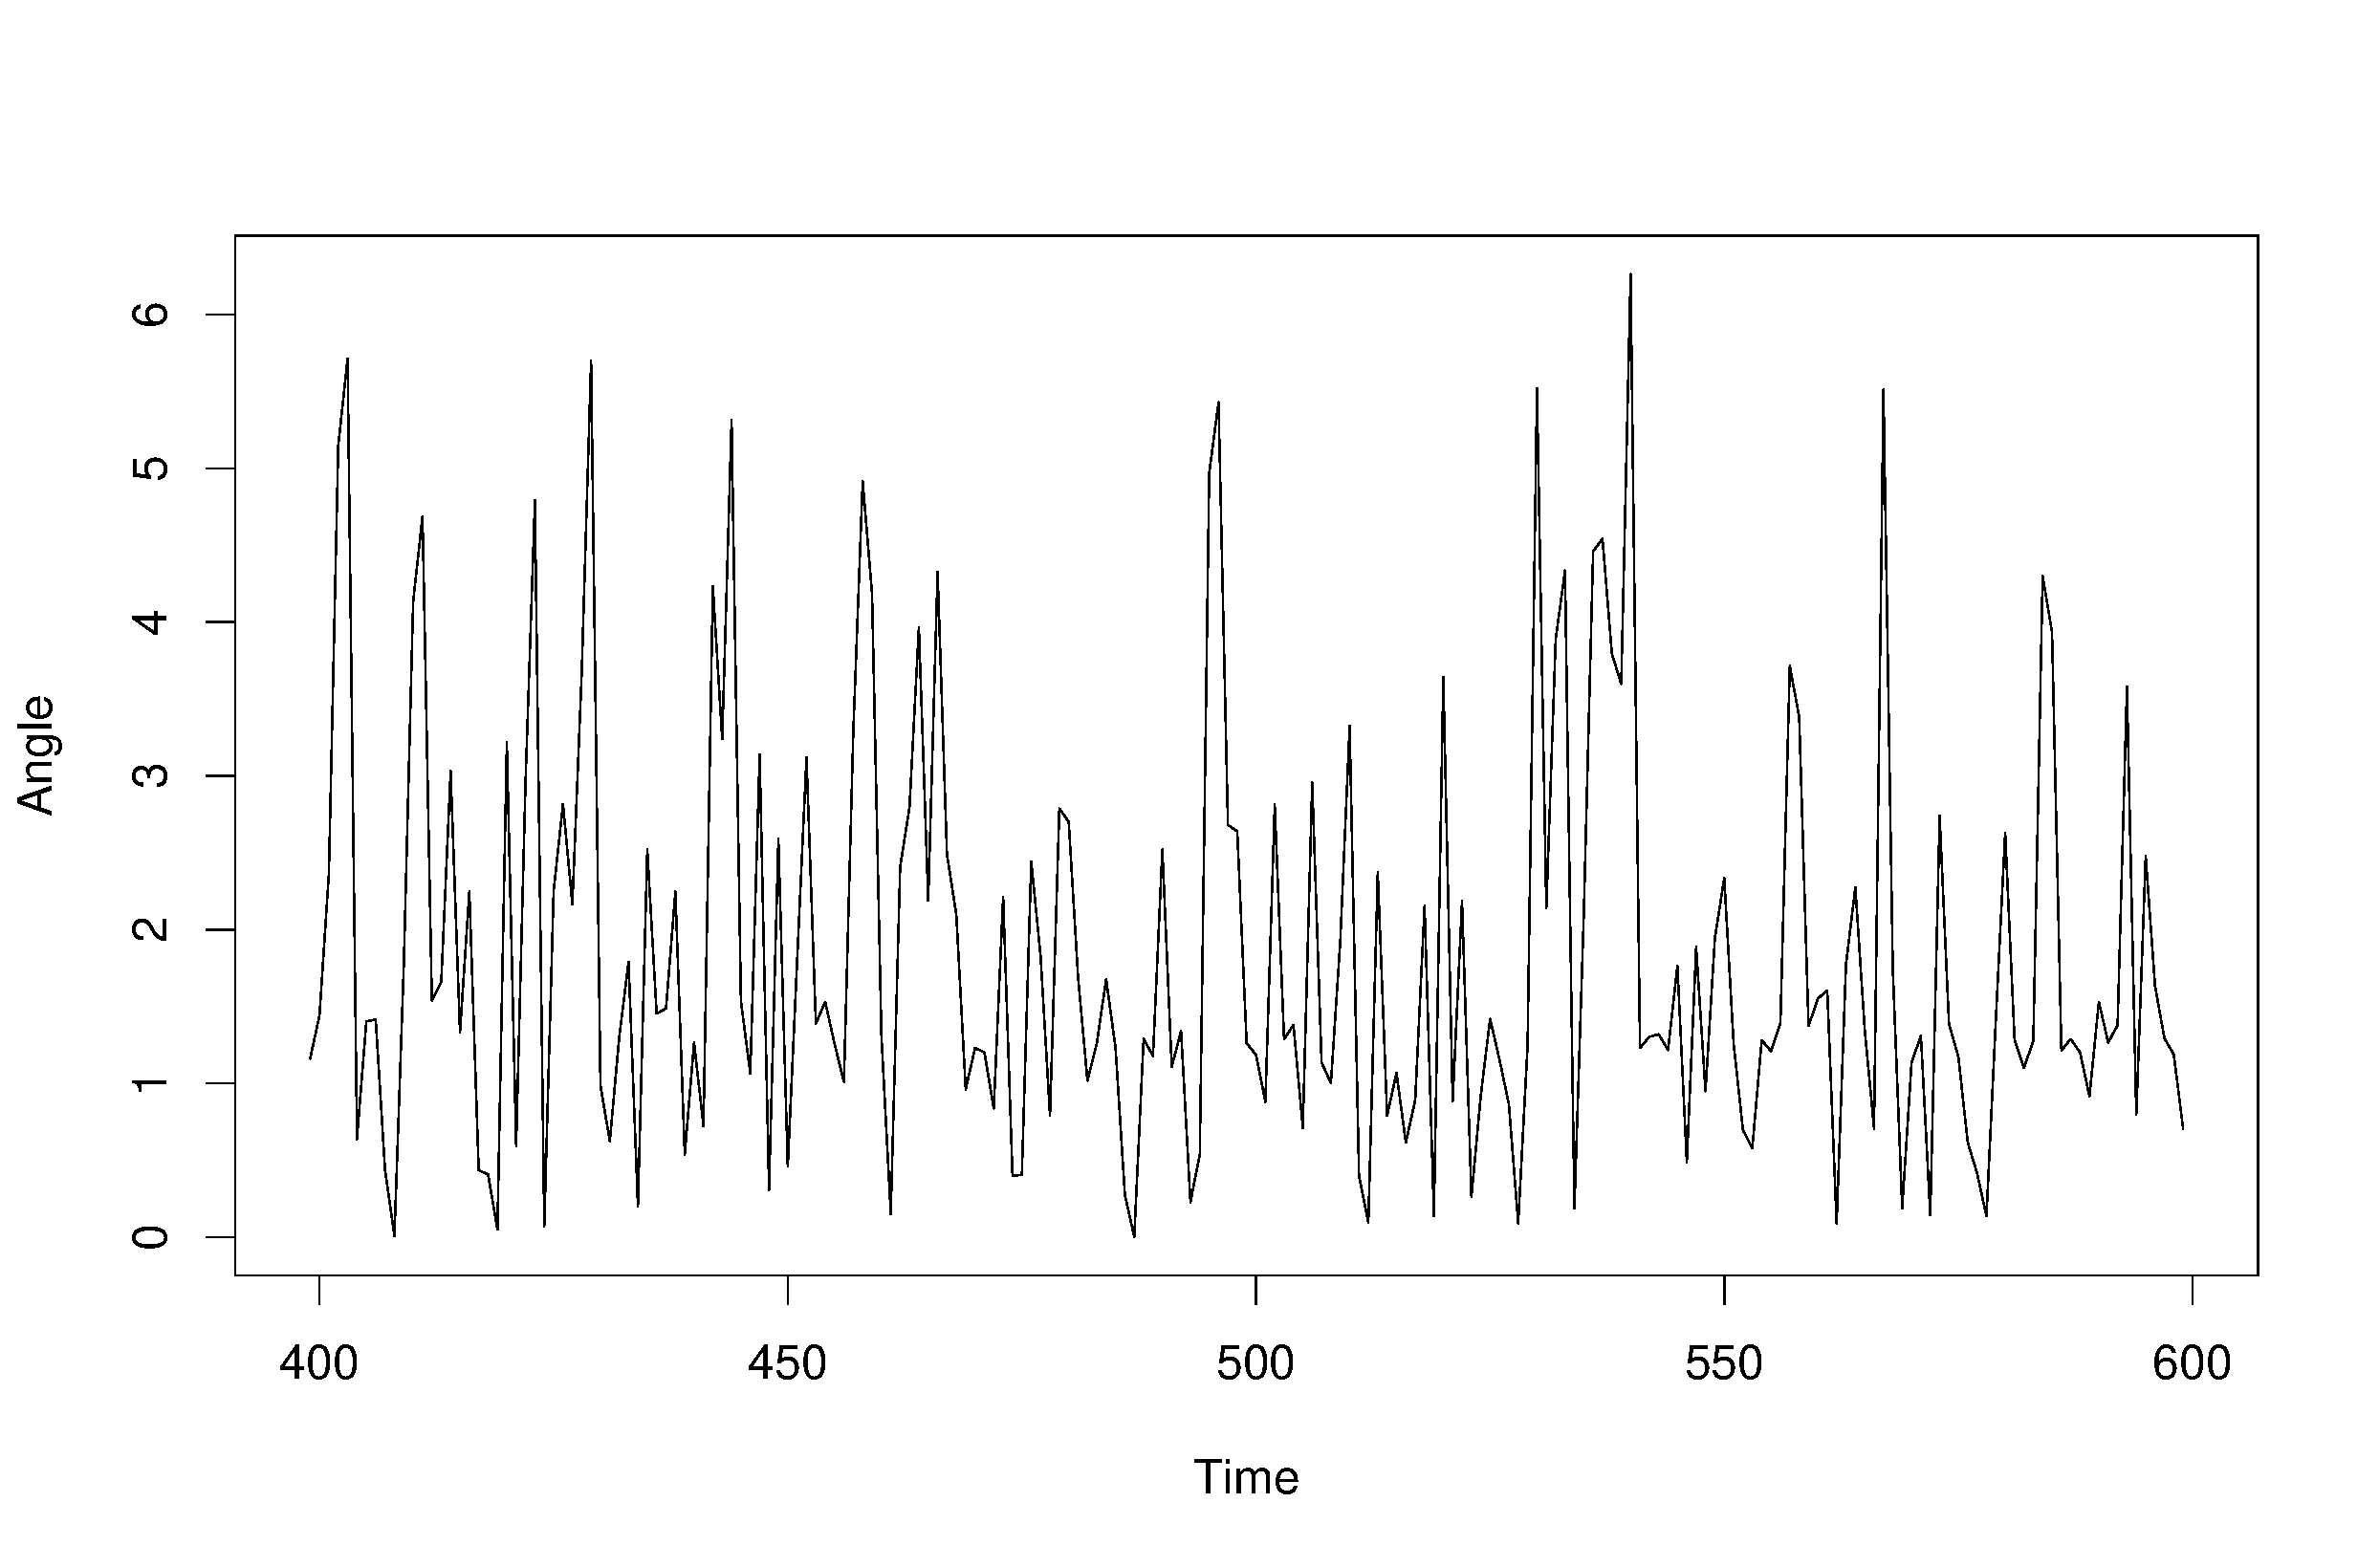
\includegraphics[width=7cm]{fig/rotation_400-600}\NN
		  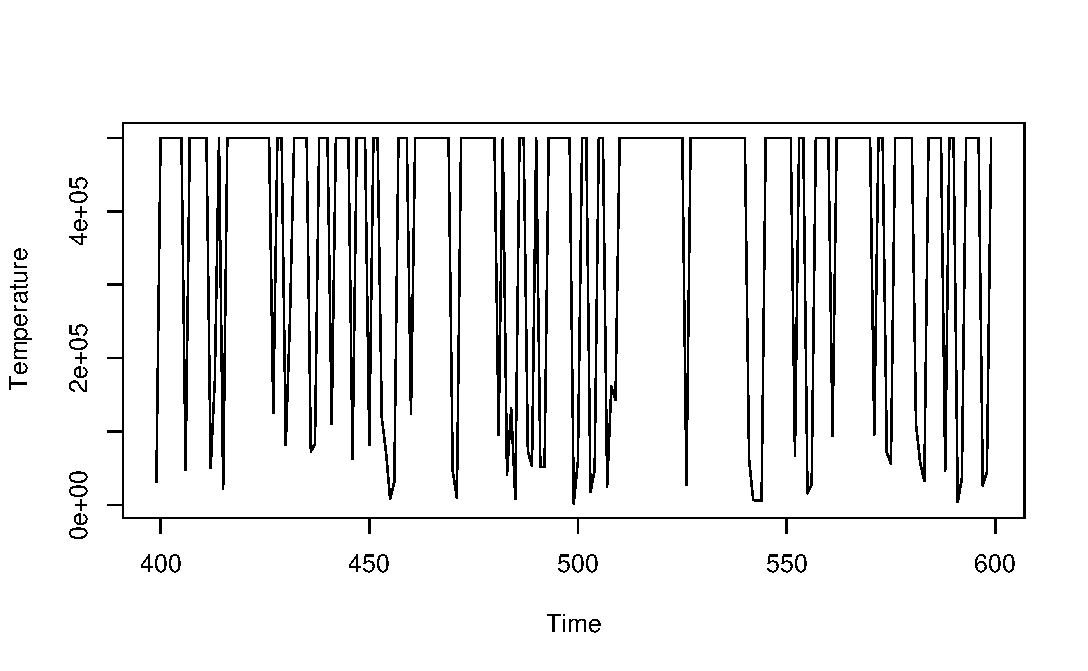
\includegraphics[width=7cm]{fig/temp_rot_400-600}\LL
		  }
\ctable[caption={The rotation at various times},
	     figure,
		  label={fig:rot19}]{c}{\tnote[]{}}{\FL
		  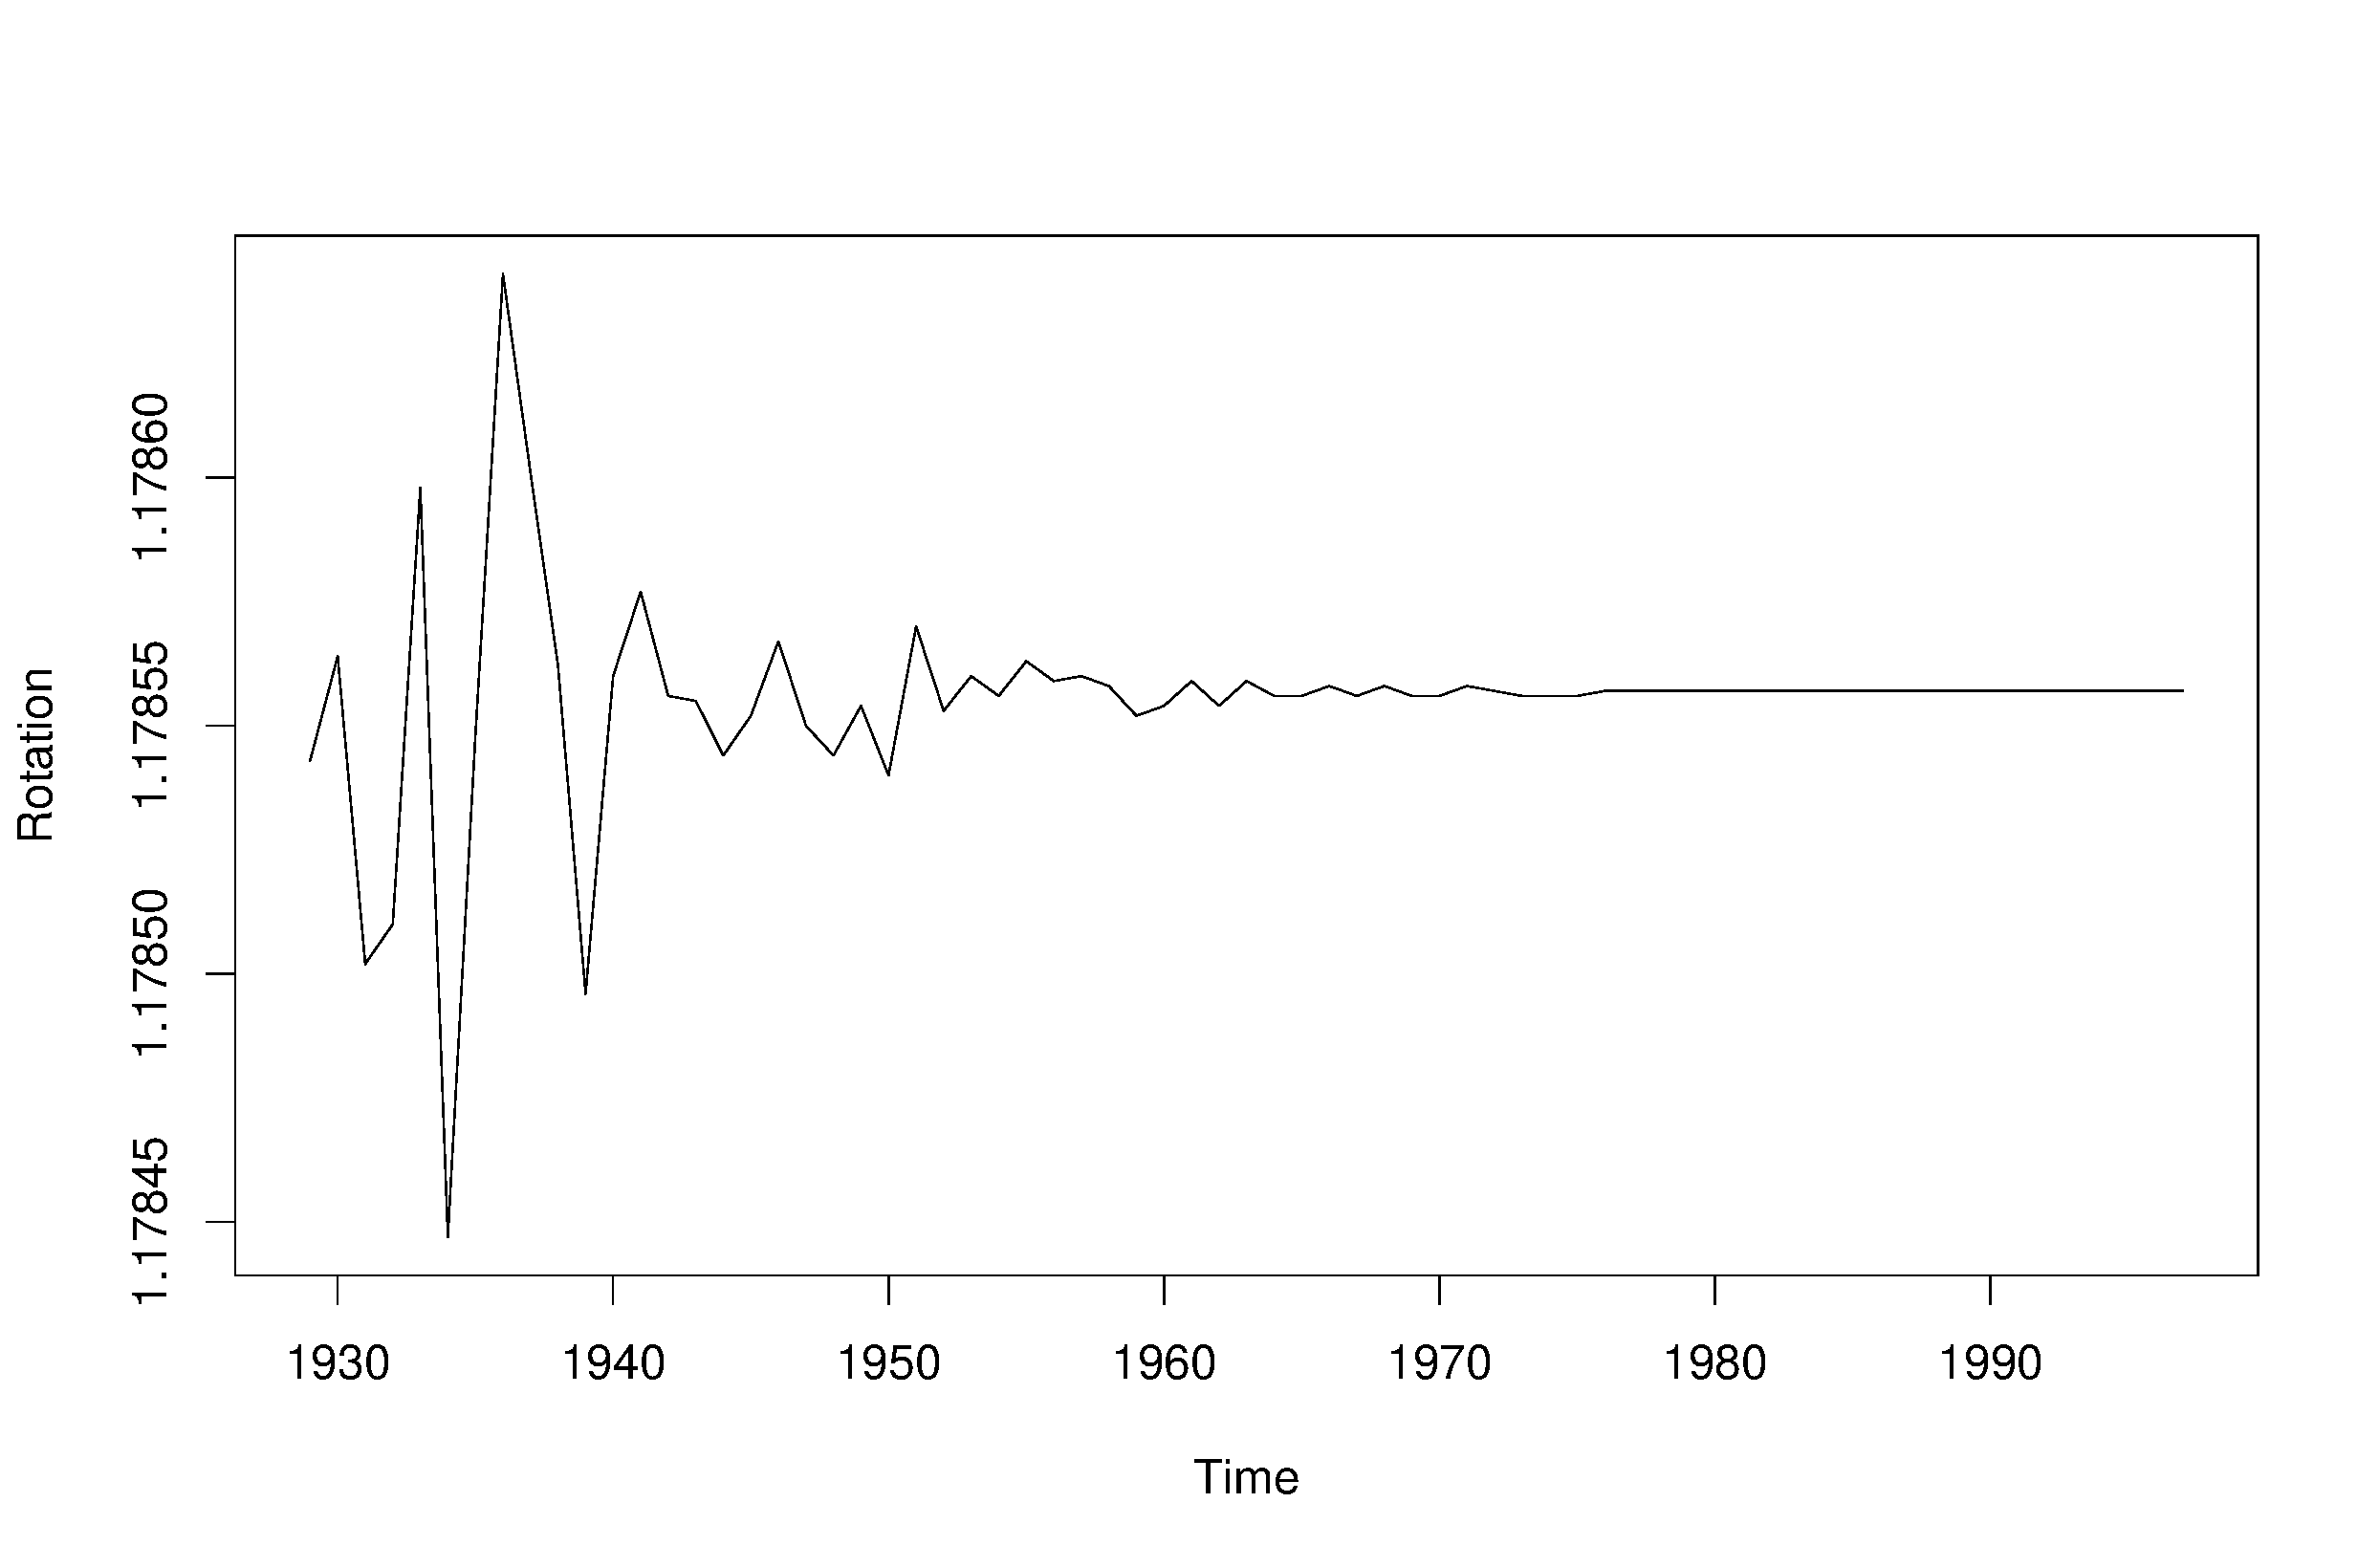
\includegraphics[width=7cm]{fig/rotation_1930-1998}\NN
		  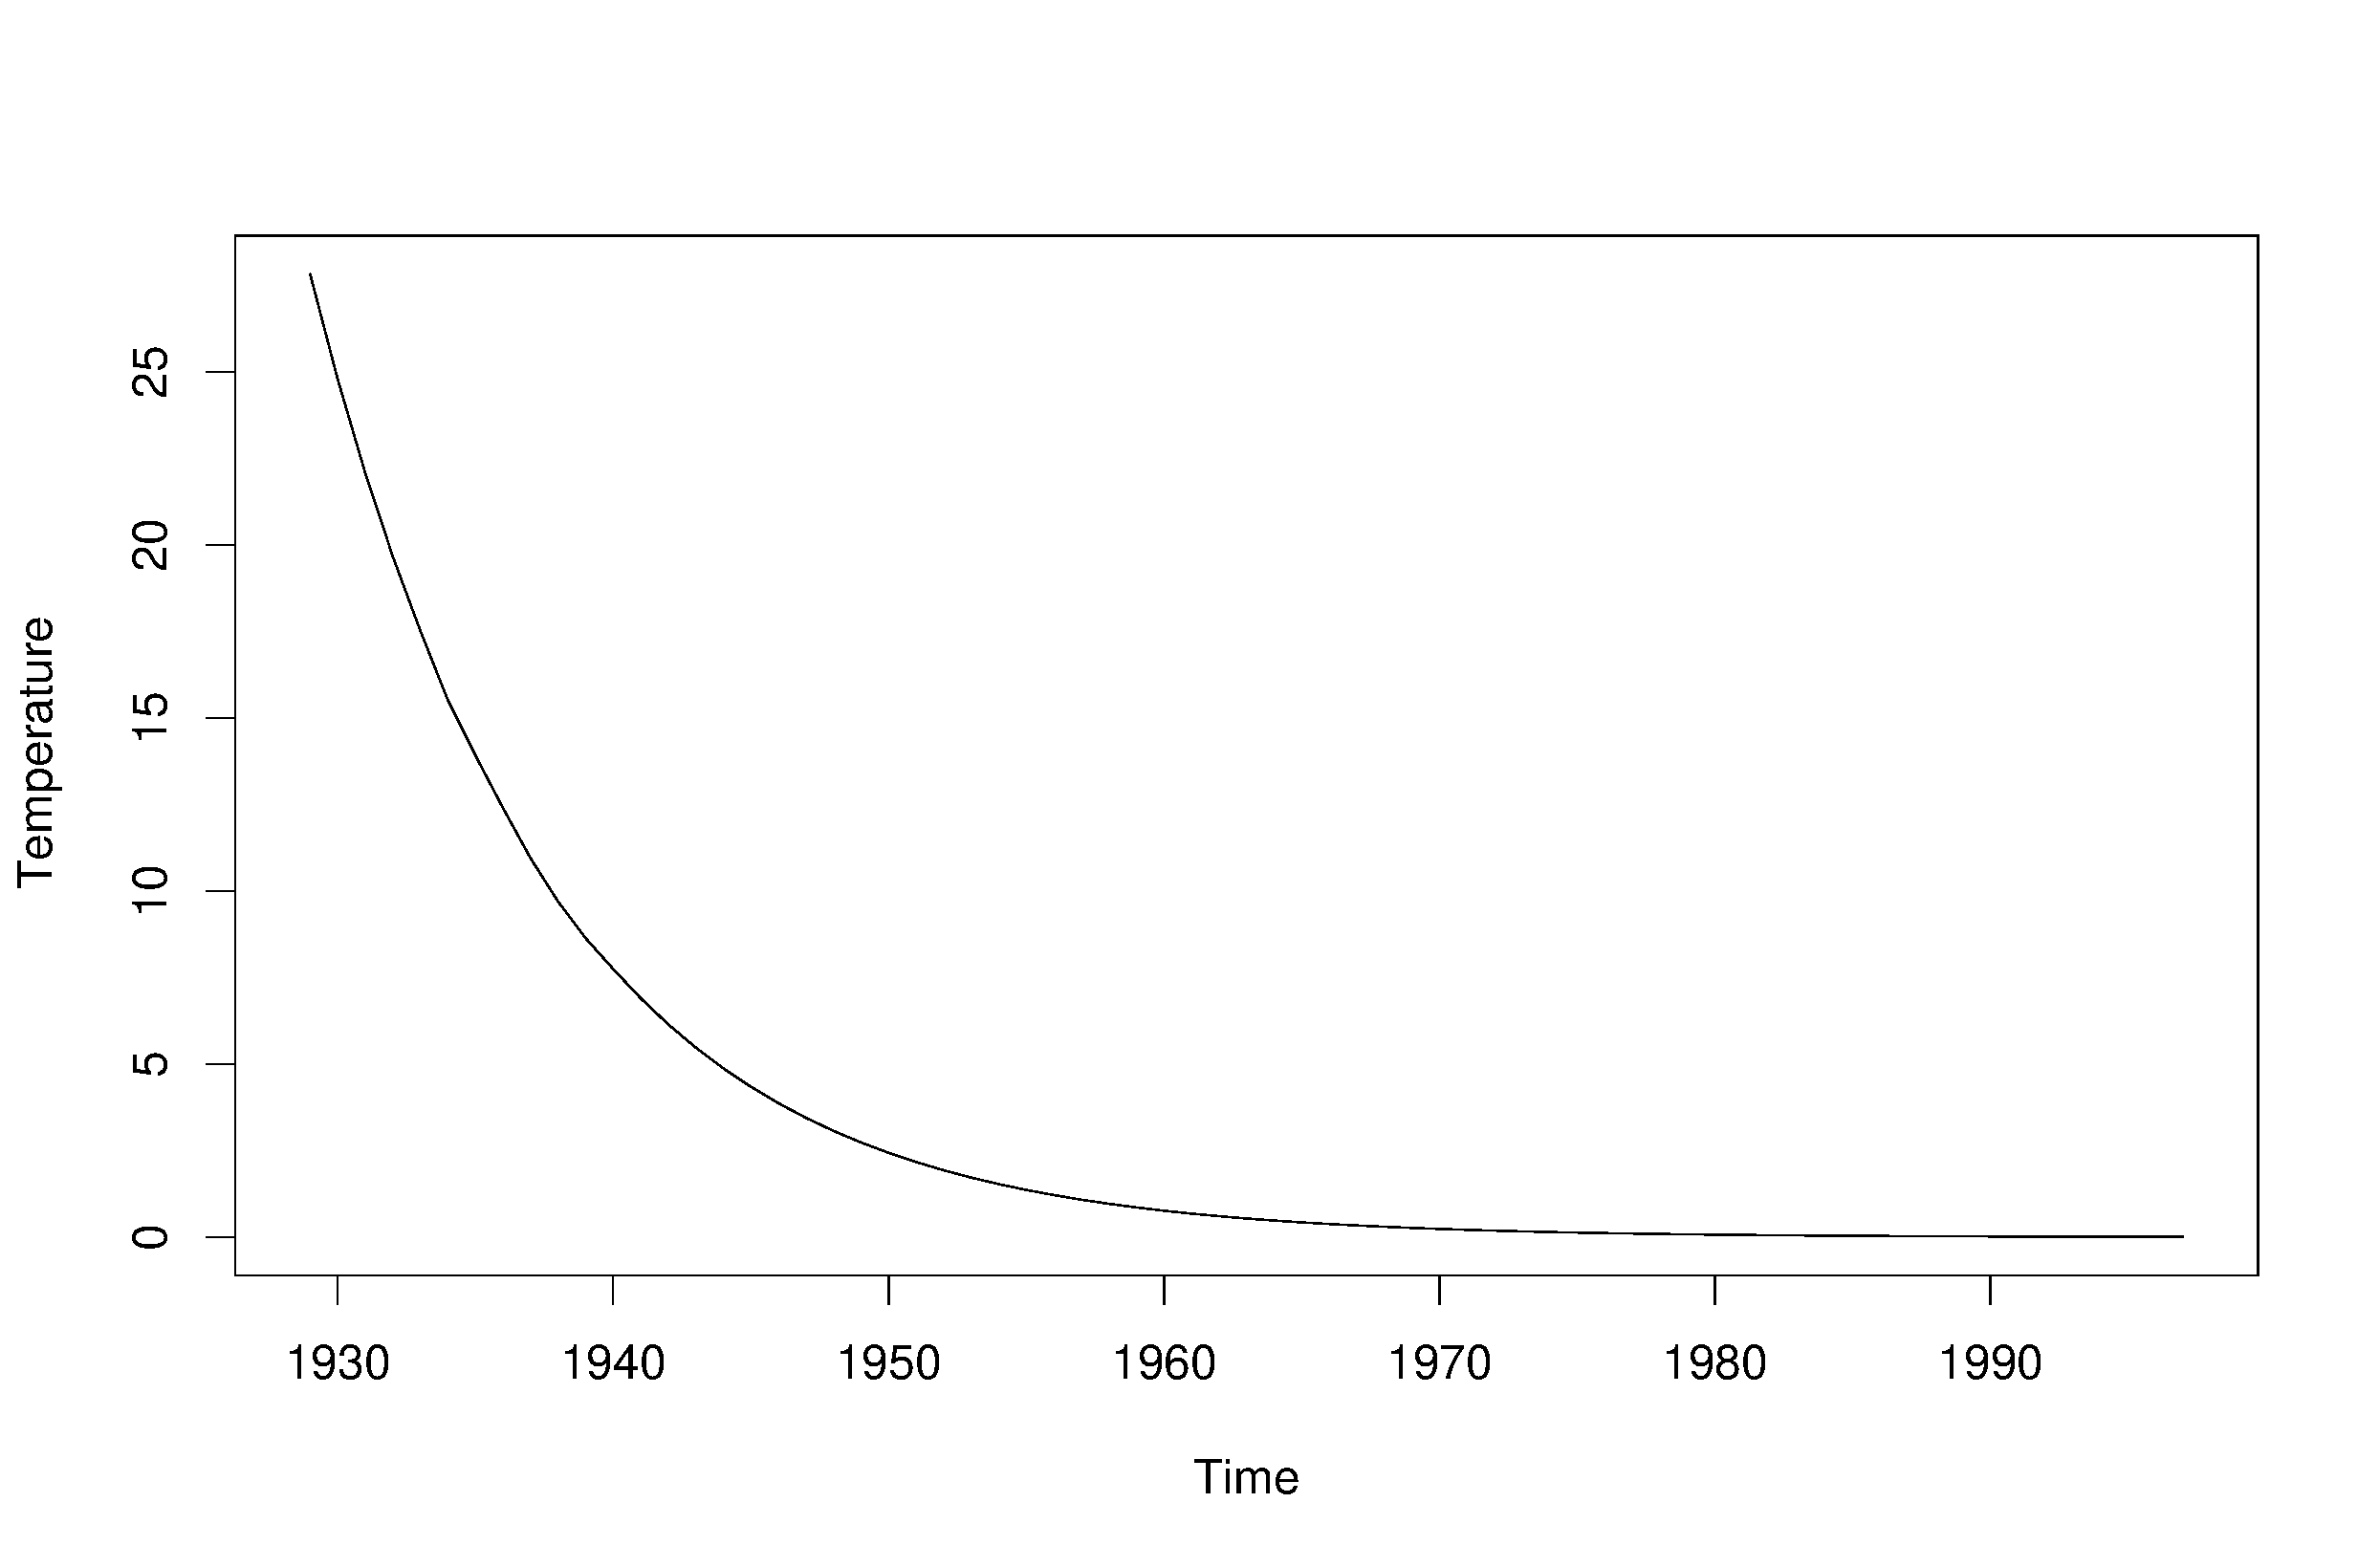
\includegraphics[width=7cm]{fig/temp_rot_1930-1998}\LL
		  }

In Fig. \ref{fig:rotful}, \ref{fig:rot46}~and \ref{fig:rot19}~the angle and
the temperature and different times is shown. The overall behaviour of the
angle over time can be seen in Fig. \ref{fig:rotful}. Equation \ref{eq:rot}~
causes the angle to behave randomly. At the beginning of the process, where
the temperature is very high, the process is very instable. This changes when
the temperature lowers. As can be seen if \ref{fig:rot46} the process seems to
`walk around' 1.2 radials. This is pure randomness. As can be seen inf Fig.
\ref{fig:rot19}~the temperature finally cools down to a minimum the movement
of the Brownian Motion also diminishes.

Perturbing the system using a Brownian Motion which influence is reduced as
the system cools, allows to jump to other angles.

\subsection{Cooling Schedule}
In the classical simulated annealing algorithm the cooling schedule has to be
fine tuned to solve each problem. However, because the renormalization
algorithm is supposed to be general purpose, we argue that fine tuning every
problem is undesirable. Therefore a auto-tuning cooling schedule is more
sensible. The thermodynamic simulated annealing algorithm proposed in
\cite{devicente2003pts}~implements a cooling schedule which uses the energy
variance and the entropy variance of the system to find a new temperature. 

\subsubsection{Energy}
As previously discussed the energy of the system is defined to be the length
of the route as found by the renormalization process. While attempting to
lower the temperature the system seeks states with a lower energy. These
states are found by perturbing the current state. When a state has a lower
energy it is accepted when
\begin{equation}\label{eq:accept}
X < e^{-\Delta E / T}
\end{equation}
where $\Delta E$ is the difference between the current energy and the last
energy, $T$ is the current temperature and $X\sim N(0, 1)$. When a state is
accepted the energy change is added to the total energy variance $E_\sigma$.
Cooling the system increases the total energy variance.

\subsubsection{Entropy}
Entropy is known in field of Physics and Information Theory. In both cases it
describes the notion of inconsistency of the current state. When the system is
at a very high temperature, --in the metallurgy analogue-- the atoms are very
unstable. When the energy and the temperature reduce the atoms will become
more stable and therefore the entropy will fall. The total entropy variance
$S_\sigma$ of the system is computed as:
\begin{equation}\label{eq:entropy}
S_\sigma = S_\sigma - \frac{\Delta E}{T}
\end{equation}
Together with the energy the entropy is used to adjust the temperature of the
system.

\subsubsection{Temperature}
When the total energy variance is large and the total entropy variance is low
the temperature can be cooled more quickly. This is reflected in a temperature
adjustment:
\begin{equation}\label{eq:tempadj}
T = \beta\frac{E_\sigma}{S_\sigma}
\end{equation}
with a adjustment factor $\beta$. This factor permits to control how long the
system stays in disequilibrium. 


% vim:ft=tex:spell spelllang=en:autoindent

